\subsection{差動駆動ロボットのオドメトリとエンコーダドリフト}

前節までに、状態を使って運動を記述し、測定できない量を推定する必要があることを見た。ここでは対象を差動駆動ロボットへ戻し、左右の車輪エンコーダだけで平面上の位置を積み上げる。ロボットには「一定の前進速度で緩やかな曲線を走る」という指令を与えている。床の上では右車輪が一部の区間でわずかに滑り、実際の軌跡と、エンコーダから積分した軌跡が少しずつ離れていく。このずれは制御の失敗だけでなく、推定を構成する最初の制約でもある。車輪の回転は測れているが、床に対する並進距離そのものは測れていないからである。

\begin{figure}[tb]
  \centering
  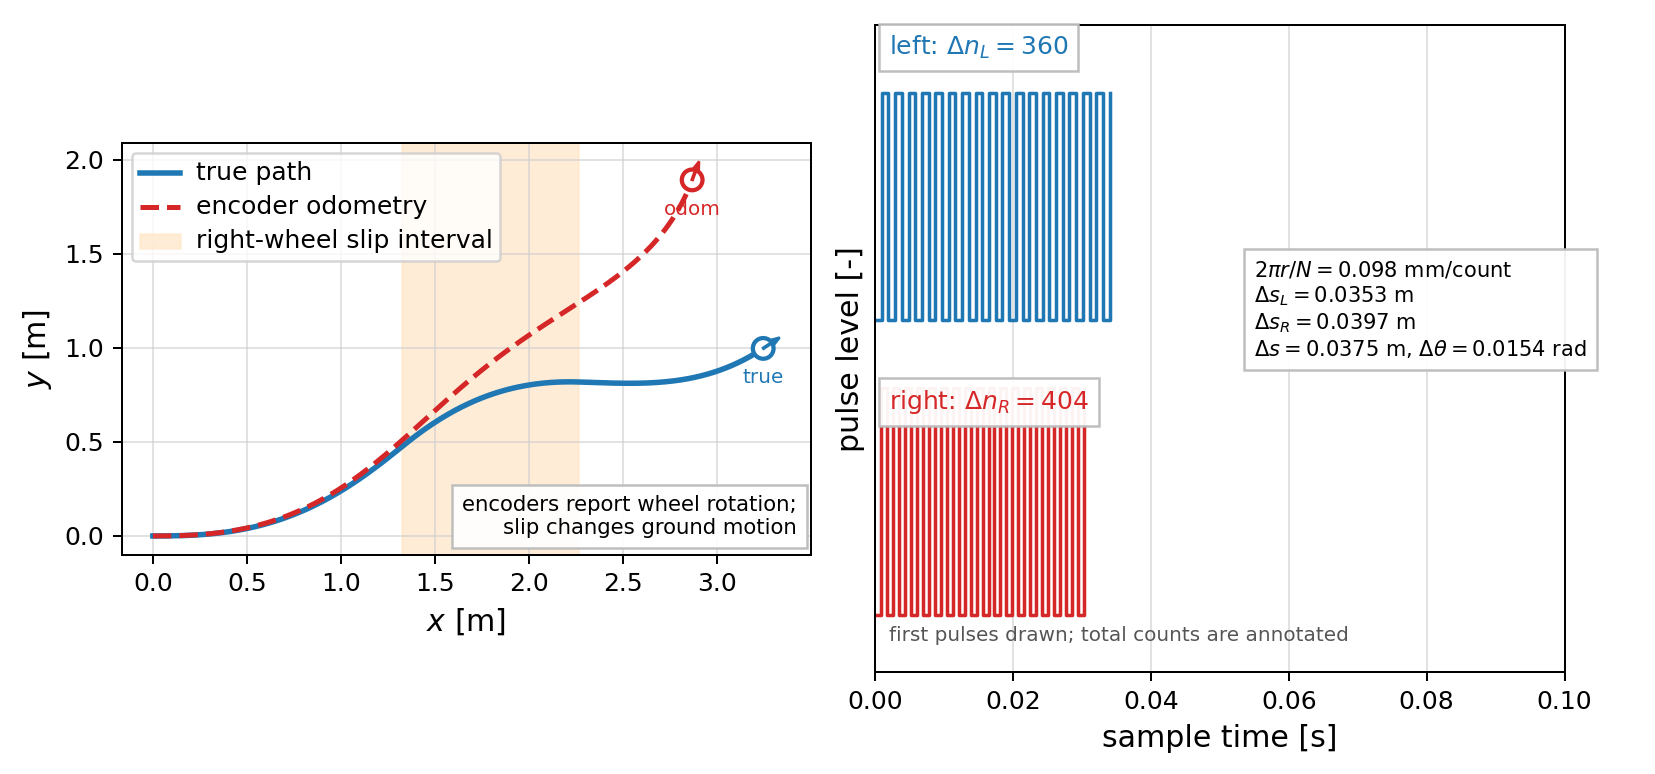
\includegraphics[width=0.95\linewidth,bb=0 0 1655 774]{figures/flow6_odometry_examples.png}
  \caption{差動駆動ロボットの真の軌跡とエンコーダオドメトリのずれ、および 1 サンプル内の左右エンコーダパルスの例。右車輪が床に対して滑ると、エンコーダは車輪の回転を数え続けるため、オドメトリは実際の床上移動より大きい右車輪距離を積分する。}
  \label{fig:flow-six-odometry-examples}
\end{figure}

図\ref{fig:flow-six-odometry-examples}の左図では、青線が床上の真の軌跡、赤破線がエンコーダから計算したオドメトリである。右車輪が滑った区間では、車輪は回っているのに床を押して進む距離が小さくなる。エンコーダはこの差を直接検出できないので、オドメトリは「車輪が地面を滑らず転がった」という仮定のもとで姿勢を更新し続ける。図が示しているのは、ミリメートル程度の車輪距離誤差でも、時間積分によってセンチメートルからデシメートル級の位置ずれに成長するという事実である。一方で、この図だけから滑りの物理原因や真の軌跡を実機上で知ることはできない。ここではシミュレーションなので青線を真値として描けるが、実機では別の測定を入れなければ、どちらの軌跡が床上の実際の動きに近いかをエンコーダだけで判定できない。

車輪半径を $r$ [m]、エンコーダの 1 回転あたりのパルス数を $N$ [count/rev] とする。サンプル時刻 $k$ から $k+1$ の間に左車輪で $\Delta n_L$ [count]、右車輪で $\Delta n_R$ [count] が数えられたとき、滑りがなく、半径の校正値も正しいという仮定のもとで、左右車輪の移動距離は
\begin{align}
  \Delta s_L&=\frac{2\pi r}{N}\Delta n_L,\\
  \Delta s_R&=\frac{2\pi r}{N}\Delta n_R
  \label{eq:wheel-pulse-distance}
\end{align}
である。係数 $2\pi r/N$ の単位は
\begin{equation}
  \frac{\mathrm{m/rev}}{\mathrm{count/rev}}
  =\mathrm{m/count}
\end{equation}
であり、パルス数を距離へ変換する換算係数になっている。たとえば $r=0.032\,\mathrm{m}$、$N=2048\,\mathrm{count/rev}$ なら
\begin{equation}
  \frac{2\pi r}{N}
  =
  \frac{2\pi\cdot0.032}{2048}
  =9.82\times10^{-5}\,\mathrm{m/count}
  =0.0982\,\mathrm{mm/count}
\end{equation}
である。

\begin{table}[tb]
  \centering
  \caption{1 サンプル $\Delta t=0.10\,\mathrm{s}$ におけるパルス数から姿勢増分までの計算例。}
  \label{tab:flow-six-encoder-step}
  \begin{tabular}{lll}
    \hline
    量 & 計算 & 値 \\
    \hline
    左車輪パルス & $\Delta n_L$ & $360\,\mathrm{count}$ \\
    右車輪パルス & $\Delta n_R$ & $404\,\mathrm{count}$ \\
    左車輪距離 & $9.82\times10^{-5}\cdot360$ & $0.0353\,\mathrm{m}$ \\
    右車輪距離 & $9.82\times10^{-5}\cdot404$ & $0.0397\,\mathrm{m}$ \\
    並進増分 & $(\Delta s_R+\Delta s_L)/2$ & $0.0375\,\mathrm{m}$ \\
    角度増分 & $(\Delta s_R-\Delta s_L)/b,\ b=0.280\,\mathrm{m}$ & $0.0154\,\mathrm{rad}$ \\
    \hline
  \end{tabular}
\end{table}

この表は、パルス数が多い右車輪のほうが長く進んだと推定され、その差が機体の向きの変化になることを数値で示している。サンプル幅で割れば車体速度と角速度も得られる。車輪間距離を $b$ [m] とし、車体中心を左右車輪の中点に置くと、サンプル内の平均速度は
\begin{align}
  v_k&=\frac{1}{2\Delta t}(\Delta s_R+\Delta s_L),\\
  \omega_k&=\frac{1}{b\Delta t}(\Delta s_R-\Delta s_L)
  \label{eq:diff-drive-kinematics}
\end{align}
である。表\ref{tab:flow-six-encoder-step}の値では
\begin{align}
  v_k&=\frac{0.0397+0.0353}{2\cdot0.10}
       =0.375\,\mathrm{m/s},\\
  \omega_k&=\frac{0.0397-0.0353}{0.280\cdot0.10}
       =0.154\,\mathrm{rad/s}
\end{align}
となる。ここで $\omega_k$ の符号は、右車輪が左車輪より長く進むと左向きに旋回するという座標系の取り方に対応している。

姿勢を $p_k=(x_k,y_k,\theta_k)$ と書く。$\theta_k$ は世界座標の $x$ 軸から見た車体前方の角度である。サンプル内で速度が一定に近いとみなせるなら、並進増分
\begin{equation}
  \Delta s_k=\frac{\Delta s_R+\Delta s_L}{2},
  \qquad
  \Delta\theta_k=\frac{\Delta s_R-\Delta s_L}{b}
\end{equation}
を使って、中点角度で
\begin{align}
  x_{k+1}
  &=x_k+\Delta s_k\cos\left(\theta_k+\frac{\Delta\theta_k}{2}\right),\\
  y_{k+1}
  &=y_k+\Delta s_k\sin\left(\theta_k+\frac{\Delta\theta_k}{2}\right),\\
  \theta_{k+1}
  &=\theta_k+\Delta\theta_k
  \label{eq:odometry-midpoint-step}
\end{align}
と積分する。この式は、車体がサンプル中に少し向きを変えることを、始点角度ではなく中点角度で代表させる近似である。たとえば $\theta_k=0.30\,\mathrm{rad}$ で表\ref{tab:flow-six-encoder-step}の増分を使うと、
\begin{align}
  x_{k+1}-x_k
  &=0.0375\cos(0.30+0.0154/2)
    =0.0357\,\mathrm{m},\\
  y_{k+1}-y_k
  &=0.0375\sin(0.30+0.0154/2)
    =0.0114\,\mathrm{m},\\
  \theta_{k+1}-\theta_k
  &=0.0154\,\mathrm{rad}
\end{align}
である。パルス数、車輪半径、車輪間距離、姿勢角がすべて具体的な単位を持つので、オドメトリは単なる幾何の公式ではなく、測定単位を姿勢単位へ変換する計算であることが明確になる。

この導出の重要な仮定は二つある。第一に、左右車輪が床に対して滑らず純転がりしていることである。第二に、半径 $r$、車輪間距離 $b$、パルス数 $N$、左右の取り付けが正しく校正されていることである。実際には、床材、加減速、旋回、荷重移動、タイヤ摩耗、左右半径差、バックラッシュ、量子化によって、$\Delta s_L,\Delta s_R$ は床上の移動距離からずれる。右車輪が $5\,\%$ だけ滑っているのにエンコーダ上は $0.040\,\mathrm{m}$ 進んだように記録されるなら、床上の右車輪距離は $0.038\,\mathrm{m}$ にしかならない。差は $0.002\,\mathrm{m}$ と小さいが、角度増分には
\begin{equation}
  \frac{0.002}{0.280}
  =0.0071\,\mathrm{rad}
  \simeq0.41^\circ
\end{equation}
として入る。これが何百サンプルも足し合わされると、位置のずれは無視できない大きさになる。

したがって、オドメトリは「短時間では強い、長時間では疑うべき」推定である。短いサンプルでは、パルス数から速度と角速度を高い時間分解能で得られる。ところが絶対位置を外部から測定していないため、滑りや校正誤差は積分で蓄積する。図\ref{fig:flow-six-odometry-examples}は、エンコーダ積分が有用であることと、エンコーダだけでは床上の真の姿勢を保証できないことを同時に示している。次に必要になるのは、車輪の回転とは別の物理量、たとえば角速度や重力方向を測るセンサであり、そこから IMU を用いた姿勢変化の推定へ進む。
